\section{Vehicle Modeling with Chronos}
\label{vehicle_modeling_chronos}

In this section we will develop and simulate vehicle model using the open source physics engine \lstinline{chronos} 


\subsection{The \lstinline{Chrono::Vehicle} library}

The \lstinline{Chrono::Vehicle} is a C++ middleware library for the modeling, simulation, and visualization of wheeled and tracked ground vehicles.
It consists of two core modules:

\begin{itemize}
\item The \lstinline{ChronoEngine_vehicle}

	\begin{itemize}
		\item Defines the system and subsystem base classes
		\item Provides concrete, derived classes for instantiating templates from JSON specification files
		\item Provides miscellaneous utility classes and free functions for file I/O, Irrlicht vehicle visualization, steering and speed controllers, vehicle and subsystem test rigs, etc.
	\end{itemize}

\item The \lstinline{ChronoModels_vehicle}
	\begin{itemize}
		\item Provides concrete classes for instantiating templates to model specific vehicle models
	\end{itemize}
\end{itemize}

The following dependencies should be satisfied in order to use the library.

\begin{itemize}
\item The \lstinline{Chrono::Engine } required
\item The \lstinline{Chrono::Irrlicht} and the \lstinline{Irrlicht} library,  \lstinline{Chrono::OpenGL} and its dependencies. Both are optional
\item The \lstinline{Chrono::FEA} and \lstinline{Chrono::MKL} (optional)
\end{itemize}

The \lstinline{Chrono::Engine } supports the notion of a system. In our case, the following components are considered a system

\begin{itemize}
\item Powertrain
\end{itemize}



\subsection{Setup simulation}
Now that we went over the basics of the \lstinline{Chrono::Vehicle} library let's try to set up a basic simulation; namely a vehicle that move in straight line.

\begin{equation}
\dot{y}\cos(\theta) - \dot{x}\sin(\theta) = 0
\end{equation} 


So, our robot can roll forward and turn while rolling, but cannot move sideways directly. We'll use this constraint to define a kinematic model for our robot. The velocity of the robot is defined by the tangent vector to its path see figure \ref{vehicle_path}. 

%\begin{figure}[!htb]
%\begin{center}
%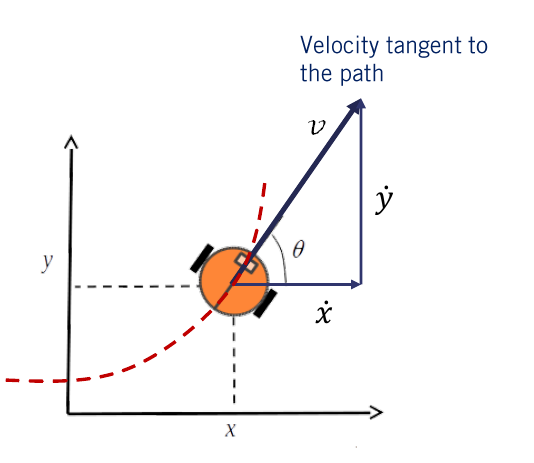
\includegraphics[scale=0.290]{img/kinematics/vehicle_path.jpeg}
%\end{center}
%\caption{Vehicle velocity.}
%\label{vehicle_path}
%\end{figure}

The following link can be used to consult for further information \lstinline{http://api.projectchrono.org/tutorial_install_project.html}












